\chapter{Data and methods}
\label{ch:datamethods}

\section{Data}
\label{sec:data}
%TODO mention data acquisition in each section
%TODO no table cause you reference each dataset

	\begin{figure}[ht]
		\centering
		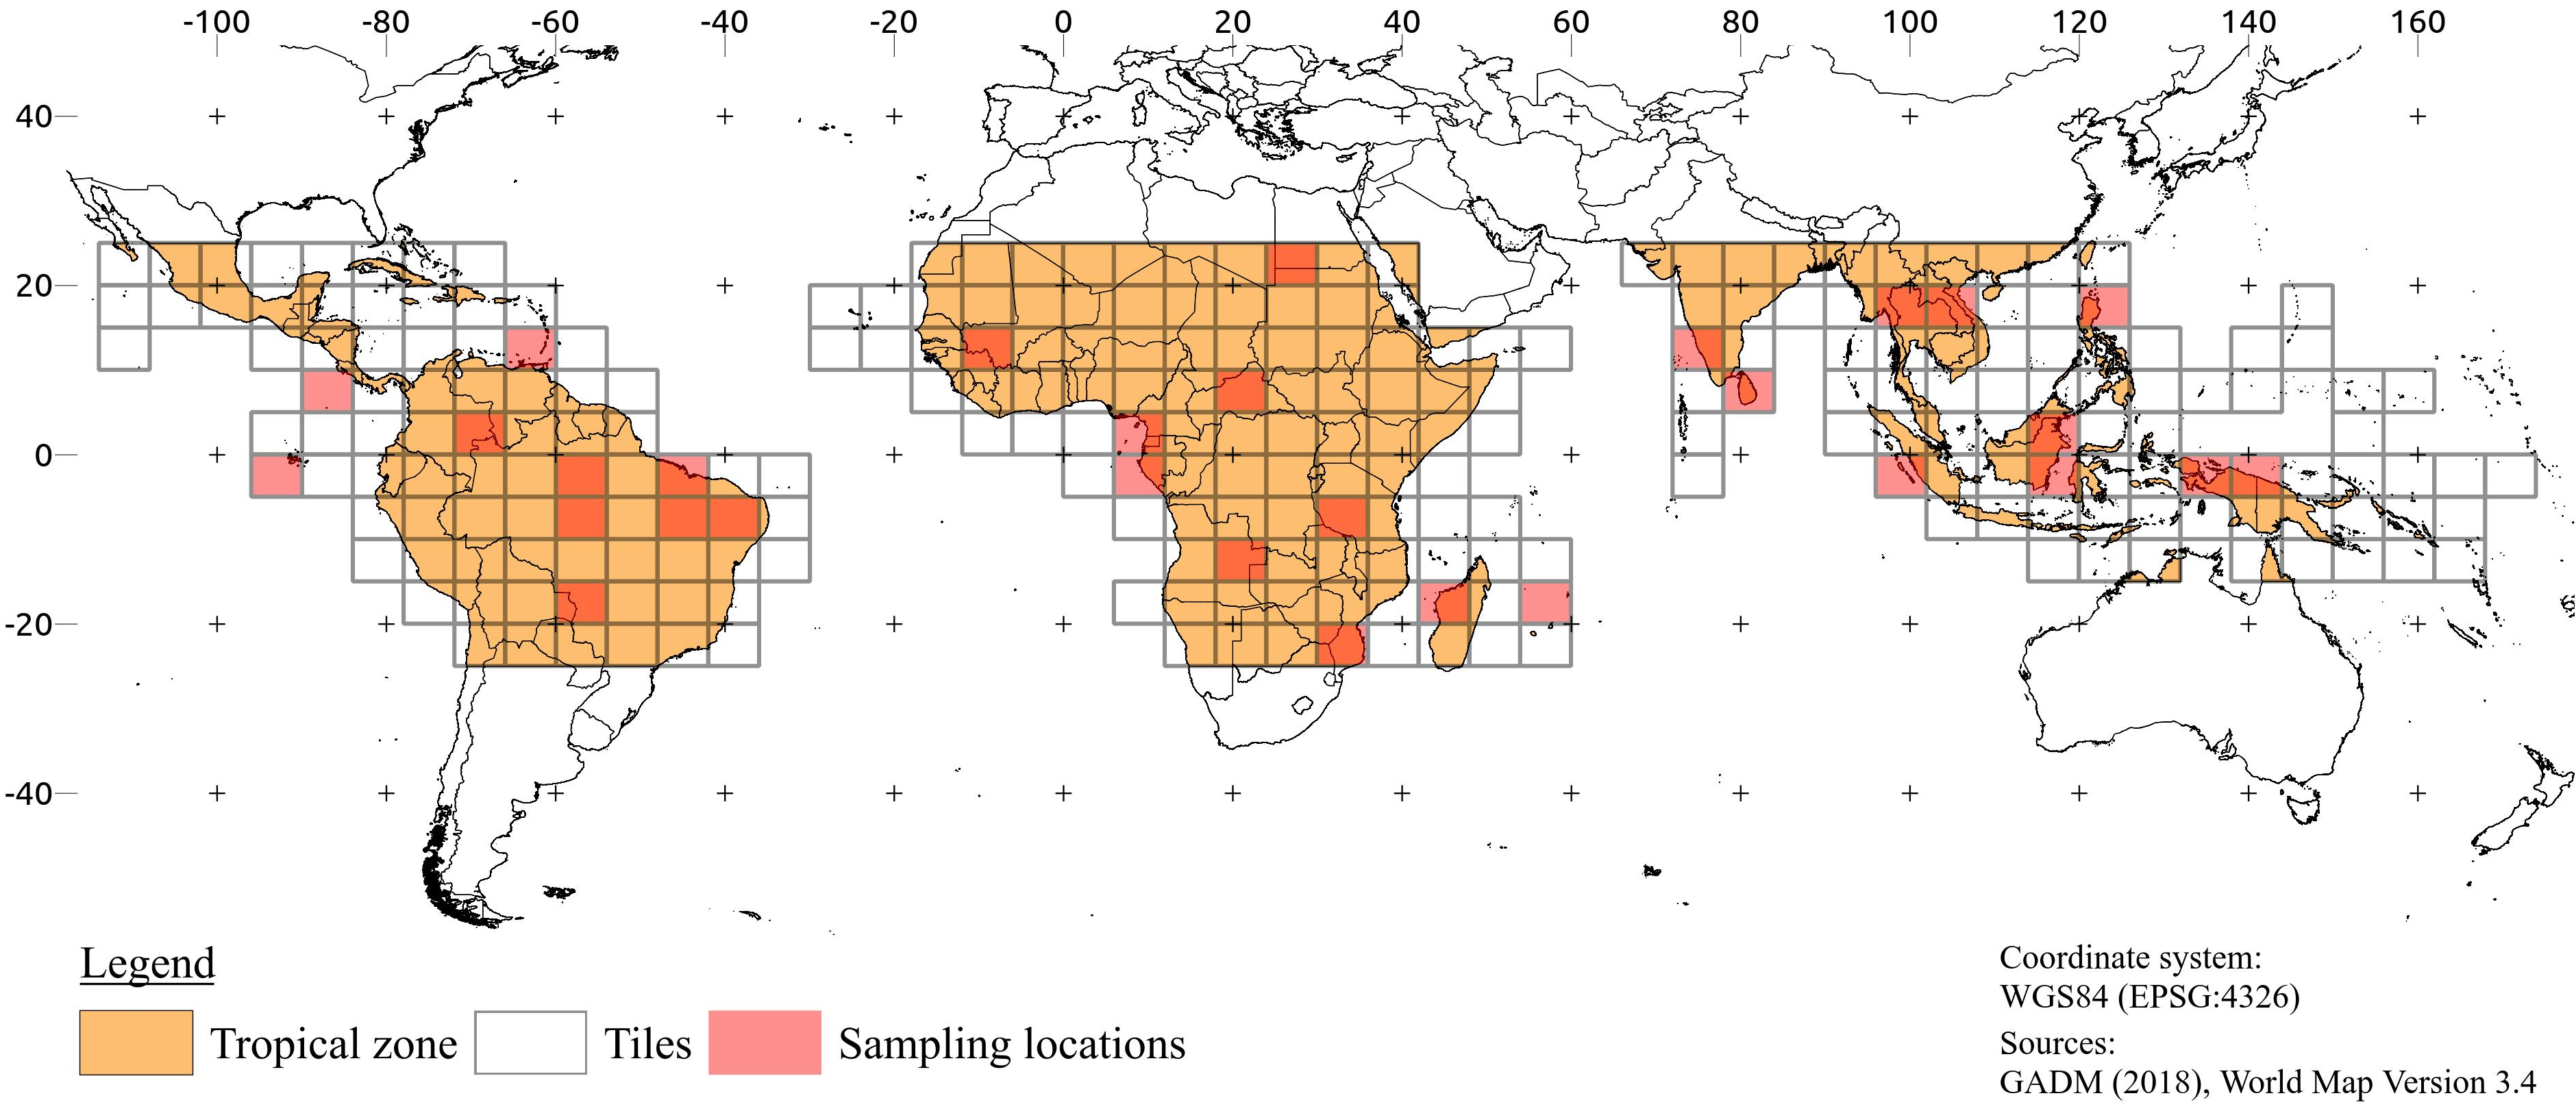
\includegraphics[scale=.97]{img/method_overview_frameless}
		\caption[Study extent]{Study extent and raster image tiles}
		\label{fig:studyextent}
	\end{figure}

	\subsection{Spatial data}
		\subsubsection{Global Forest Change}
			\ac{GFC} 2000-2012 Version 1.0 is the first high resolution dataset that provides a comprehensive view on the annual global forest cover change between 2000 and 2012 (\citet{Hansen2013, Li2017}). The initial \ac{GFC} dataset released by \citeauthor{Hansen2013} is extended by recent releases which encompass the annual forest cover changes between 2000-2013, 2000-2014, 2000-2015 and 2000-2016, respectively. All versions of this dataset have in common, that they are derived from growing season imagery captured by the remote sensing satellite Landsat 7 Enhanced Thematic Mapper Plus (ETM+) at a spatial resolution of 30 meters per pixel (\citet{Hansen2013a}). On the satellite imagery a time-series spectral metrics analysis is applied to gather the global forest extent at 2000 as well as the annual forest loss and gain. Hence, \ac{GFC} comprises three independent data layers  tree cover, annually forest loss and  forest gain divided into 10x10 degree tiles by the geodetic coordinate system World Geodetic System 1984 (EPSG:4326). Furthermore, across the provided layers the pixel data is coded in unsigned 8 bit integers. Hansen et al. defined trees as all vegetation taller than 5 meters for their study. Forest loss is defined as a stand displacement disturbance leading from a forest state to a non forest-state. To compute this losses.
		\subsubsection{GlobeLand30}
			\lipsum[1-2]
		\subsubsection{Intact Forest Landscapes}
			\lipsum[1-2]
		\subsubsection{Aboveground Woody Biomass}
			\lipsum[1-2]
		\subsubsection{Global Soil Organic Carbon}
			\lipsum[1-2]
		\subsubsection{Auxiliary}
			\lipsum[1-2]

	\subsection{Empirical data}
		\subsubsection{Soil Organic Carbon}
			\lipsum[1-2]
		\subsubsection{Ecosystem Service Values}
			\lipsum[1-2]


\section{Methods}
\label{sec:methods}
%TODO need more speacking section headings
%TODO flowchart

	\subsection{Pre-processing}
		\lipsum[1-2]

	\subsection{Deforestation}
		\subsubsection{Forest definition}
			\lipsum[1-2]
		\subsubsection{Land use change driver}
			\lipsum[1-2]
		\subsubsection{Accuracy assessment}
			\lipsum[1-2]

	\subsection{Emissions}
		\subsubsection{Above ground biomass}
			\lipsum[1-2]
		\subsubsection{Soil organic carbon change}
			\lipsum[1-2]

	\subsection{Ecosystem service values}
		\subsubsection{Ecosystem service value loss}
			\lipsum[1-2]
		\subsubsection{Ecosystem service value gain}
			\lipsum[1]

	\subsection{Binning analysis}
		The previous sections were focused on the generation of large scale spatial data. Now, a feasible method must be developed for analyzing, aggregating, interpreting and visualizing the output data. To develop a good approach we must formalize the problem domain. At first we are confronted with large N (many samples) which results in many variables (dimensionality) and complexity of relationships among this variables \citep{Carr1990}. From a visual/analytical perspective georeferenced raster maps can be interpreted as a multivariate scatter plot of large datasets where longitude and latitude represent the x and y coordinate of an data point and the pixel values (in this case nominal scaled) representing the third dimension as an group coloring. Therefore we have a large multidimensional dataset combined with a scatter plot visualization which leads commonly to over plotting issues and hidden point densities \citep{Carr1987}. Due to the spatial nature of your data we are also confronted with not equal distributed data some regions show high data densities and other regions have spares to no data. Also a severe problem domain is the frame size of our representation. Goal is to present data on a continental level which intensifies visual problems. Each pixel has a resolution of approximately 30x30m, the continental representation of americas spanning approximately 1200000x120000km2. Therefore small scale isolated changes are hidden and only large scale changes are visual detectable. Which results in hidden details and not perceivable patterns of change.

		Goal should be to develop an process who solve this issues and generates satisfying output for our multivariate data. In case of raster data a re-sampling to coarser resolution could solve over plotting and resolution issues as well normalize the unequal distributed data. But the nature of re-sampling (for nominal data a nearest neighbor or majority wins \note{Reference}) would negate important spatial patterns as well frequency distributions. Another well known approach is to use binning of the spatial explicit data with a certain kind of regular polygon that is tessellating the plane \citep{Carr1992}. Polygon tessellations provide numerous opportunities for presenting multivariate statistical summaries. The scaling of the polygon could be used to represent pixel densities within the polygon area, a polygon filling color gradient is applicable to show nominal or ordinal scaled data. Also it is imaginable to use the polygon interior for a pie chart. To use regular tessellation it is important to mention there are only three types of regular polygons tessellate the plane: squares, equilateral triangles and hexagons \citep{Carr1992}. Square tessellation is the most common approach used for binning in spatial visualization. A raster image is a square tessellation. In a square mosaic each polygon shares 4 edge neighbors and 4 vertex neighbors \note{more explanation error distance disadvantages etc}. \note{Hexagons properties, advantages disadvantages of both tessellations, what are your visuals scaled and pie, mention polygon literature}

		To be flexible at hexagon construction we accept 4 different parameters as construction arguments: $D$ long diagonal (Diameter of the circumscribing circle), $d$ short diagonal (diameter of the inscribed circle), $A$ area the hexagon should span and or $e$ the edge length. One selected parameter of these is used to compute $R$ the radius of the circumscribing circle with respect to input parameter as shown in  equation \ref{eq:paramters}. R is used to calculate the midpoint $<c_x, c_y>$ of the hexagon located in the first quadrant of the cartesian coordinate system Equation \ref{eq:centerx} and \ref{eq:centery}. Equation \ref{eq:hexagon} shows the computation of the hexagon anti-clockwise vertex matrix. Whereas the two leftmost vertices (first and last row of the matrix $\textbf{H}$) are located at koordinatenursprung, will sagen auf deutsch korridanten at x=0 und y=value of matrix. In summary equation \ref{eq:paramters} to \ref{eq:hexagon} show the creation of an hexagon at the leftmost corner of first quadrant. The orientation is important for the subsequent mosaic creation.
		\begin{equation}
		\label{eq:paramters}
			R = \frac{\sqrt{2A}}{\sqrt[4]{27}} = \frac{D}{2} = \frac{d}{\sqrt{3}} = e
		\end{equation}
		\begin{equation}
		\label{eq:centerx}
			c_x = \frac{R\sqrt{3}}{2} 
		\end{equation}
		\begin{equation}
		\label{eq:centery}
			c_y = R
		\end{equation}
		\begin{equation}
		\label{eq:hexagon}
			\mathbf{H} =
			\begin{bmatrix}
				0 & c_x & 2c_x & 2c_x & c_x & 0 \\
				R\sin\left(\frac{7\pi}{6}\right) + c_y & 0 & R\sin\left(\frac{11\pi}{6}\right)+c_y & R\sin\left(\frac{\pi}{6}\right)+c_y & 2R & R\sin\left(\frac{5\pi}{6}\right)+c_y \\
				1 & 1 & 1 & 1 & 1 & 1
			\end{bmatrix}
		\end{equation}
		A polygon tessellation needs several polygons to create a grid in case of the creation of one hexagon with the presented algorithm needs approximately \note{benchmark} but the creation of \note{several N hexagons} needs approximately \note{benchmark}. Therefore it is much simpler to create only one hexagon with the presented algorithm and to create the grid polygons by copying the coordinates of the source polygon and translating them to their target position with a affine transformation matrix shown in equation \ref{eq:translate}. To create the grid we get the rectangular bounds of the area to tessellate as a matrix $\textbf{B} \in R^{2\times2}$ (equation \ref{eq:bounds}), where the first column of the matrix contains the lower left corner and the second column the upper right corner of the image. Each subsequent translation in regards of $x_{off}$ is $x_1 + d $
		\begin{equation}
		\label{eq:translate}
		\mathbf{T} =
			\begin{bmatrix}
				1 & 0 & x_{off} \\
				0 & 1 & y_{off} \\
				0 & 0 & 1
			\end{bmatrix} \circ \mathbf{H}
		\end{equation}
		\note{Here comes the description of the segmentation process} 
		\begin{equation}
		\label{eq:bounds}
			\mathbf{B} =
			\begin{bmatrix}
				x_1 & x_2 \\
				y_1 & y_2
			\end{bmatrix}
		\end{equation}
		\begin{equation}
		\label{eq:radius}
			R = \frac{\sqrt{2A}}{\sqrt[4]{27}}
		\end{equation}
		\begin{equation}
		\label{eq:percentage}
			y = \frac{P(y_2-y_1)}{100} + y_1
		\end{equation}
		\begin{equation}
		\label{eq:left}
			f^{-1}(y) =
			\begin{cases} 
				-\frac{y - y_1}{\tan{(\frac{\pi}{6}})} + \frac{x_1 + x_2}{2} & \text{if } y_1 \le y < y_1 + R\sin{(\frac{5\pi}{6})} \\
				x_1 & \text{if } y_1 + R\sin{(\frac{5\pi}{6})} \le y < R(\sin{(\frac{5\pi}{6})} + 1) \\
				\frac{y - y_2}{\tan{(\frac{\pi}{6}})} + \frac{x_1 + x_2}{2} & \text{if } R(\sin{(\frac{5\pi}{6})} + 1) \le y \le y_2
			\end{cases}
		\end{equation}
		\begin{equation}
		\label{eq:right}
			g^{-1}(y) = 
			\begin{cases} 
				\frac{y - y_1}{\tan{(\frac{\pi}{6}})} + \frac{x_1 + x_2}{2} & \text{if } y_1 \le y < y_1 + R\sin{(\frac{5\pi}{6})} \\
				x_2 & \text{if } y_1 + R\sin{(\frac{5\pi}{6})} \le y < R(\sin{(\frac{5\pi}{6})} + 1) \\
				-\frac{y - y_2}{\tan{(\frac{\pi}{6}})} + \frac{x_1 + x_2}{2} & \text{if } R(\sin{(\frac{5\pi}{6})} + 1) \le y \le y_2
			\end{cases}
		\end{equation}
		\begin{equation}
		\label{eq:line}
			\mathbf{L} =
			\begin{bmatrix}
				f^{-1}(y) & g^{-1}(y) \\
				y & y
			\end{bmatrix}
		\end{equation}
		\note{Need alternative computational not so intensive approach, do it} 
	\begin{figure}[ht]
		\centering
		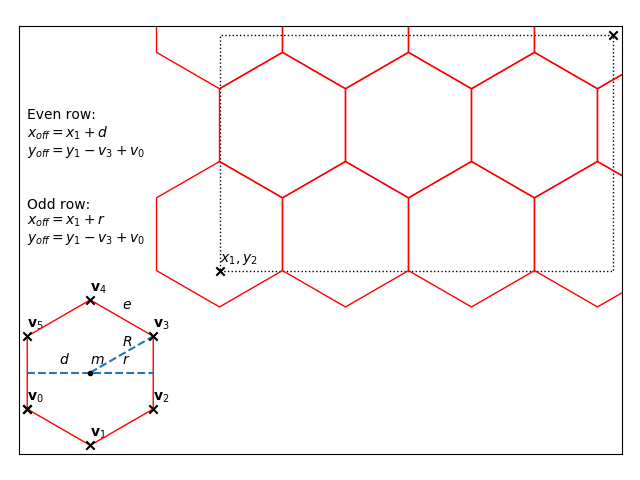
\includegraphics[scale=.9]{img/hexagons}
		\caption[Study extent]{Study extent and raster image tiles}
		\label{fig:studyextent}
	\end{figure}
